\documentclass[conference]{IEEEtran}
\IEEEoverridecommandlockouts

\usepackage{cite}
\usepackage{amsmath,amssymb,amsfonts}
\usepackage{algorithmic}
\usepackage{graphicx}
\usepackage{textcomp}
\usepackage{xcolor}

\def\BibTeX{{\rm B\kern-.05em{\sc i\kern-.025em b}\kern-.08em
    T\kern-.1667em\lower.7ex\hbox{E}\kern-.125emX}}

\begin{document}

\title{Comparative Analysis of Q-learning and SARSA in the Flappy Bird Game}


\author{\IEEEauthorblockN{1\textsuperscript{st} Kha Duy Phan}
\IEEEauthorblockA{\textit{Université Côte d'Azur, France} \\
duy-kha.phan@etu.univ-cotedazur.fr}
\and
\IEEEauthorblockN{2\textsuperscript{nd} Huy Dinh Nguyen}
\IEEEauthorblockA{\textit{Université Côte d'Azur, France} \\
dinh-huy.nguyen@etu.univ-cotedazur.fr}
}

\maketitle

\begin{abstract}
This report analyzes the performance of Q-learning and SARSA in training an agent for the Flappy Bird game. An enhanced reward function is designed to encourage prolonged flight, optimize gift collection, reward strategic actions, and penalize collisions. The study covers game mechanics, state representation, action dynamics, reward structure, learning algorithms, and experimental evaluation, with insights on performance, gift acquisition efficiency, and potential future improvements.
\end{abstract}

\begin{IEEEkeywords}
Reinforcement Learning, Q-learning, SARSA, Flappy Bird, Reward Functions.
\end{IEEEkeywords}

\section{Introduction}
% Reinforcement Learning has been widely applied in training agents for sequential decision-making tasks. This report explores the effectiveness of Q-learning and SARSA in optimizing an agent’s performance in Flappy Bird, a continuous control task requiring precise navigation. The agent must avoid pipes, maximize survival time, and collect gifts, which serve as additional incentives in the learning process.

Reinforcement Learning (RL) is extensively used to train agents for sequential decision-making problems. In Flappy Bird, a side-scrolling game, the agent controls a bird that moves forward while being influenced by gravity. The only available action is flapping, which briefly increases the bird's upward velocity. The primary goal is to maneuver through dynamically placed pipe gaps while avoiding collisions to maximize both survival time and score.

Beyond obstacle avoidance, the agent can also collect gifts that spawn at different locations along its flight path. These gifts offer bonus rewards, incentivizing exploration of alternative flight strategies. However, acquiring them introduces a trade-off between risk and reward, as adjusting the trajectory to obtain gifts may increase the likelihood of crashes.

\section{Game Description and Mechanics}

\subsection{Game Elements and Dynamics}
\begin{itemize}
    \item \textbf{Visual Elements:} The game features a background, moving ground, pipes as obstacles, and a bird controlled by the agent. A bonus element, referred to as a “gift”, is also included.
    \item \textbf{Dynamics:}
    \begin{itemize}
        \item The bird is affected by gravity and can flap to gain altitude.
        \item Pipes continuously move leftwards at a constant speed, with new pipes generated as the older ones exit the screen.
        \item The gift moves along with the pipes; when collected, it provides an extra reward.
    \end{itemize}
\end{itemize}

\subsection{State Representation and Actions}
The agent's perception of the environment is defined by its state representation and the available actions.

\subsubsection{State Representation}
The positions of the bird, pipes, and gifts are represented by their respective (x,y) coordinates. Notably, the bird's x-coordinate remains constant. The state of the game is represented as a tuple capturing essential information related to the bird's position and the environment:
\begin{itemize}
    \item \textbf{X-coordinate of the next pipe}
    \item \textbf{Vertical distance to the next pipe:} The difference in height between the bird and the lower edge of the upper pipe
    \item \textbf{X-coordinate of the next gift}
    \item \textbf{Vertical distance to the next gift:} The difference in height between the bird and the gift
\end{itemize}
Due to the continuous nature of the game, representing each state at the pixel level would result in an excessively large state space, making learning inefficient. To address this, the game environment is divided into discrete areas, where each area groups multiple pixel positions together. The agent considers all states within the same area as equivalent and applies the same action policy. 

This discretization reduces complexity, accelerates learning, and enables more effective generalization across similar game scenarios. By mapping the bird’s position, pipes, and gifts to predefined grid-like areas, the agent can make consistent decisions without the need for an impractically large state space.

\subsubsection{Actions}
Action selection is implemented using greedy strategy. Accordingly, the agent has two possible actions:
\begin{itemize}
    \item \textbf{Action 0 (do nothing):} The bird is allowed to descend naturally under gravity.
    \item \textbf{Action 1 (flap):} The bird flaps its wings to gain altitude, counteracting gravity.
\end{itemize}

\subsection{Enhanced Reward Function}
The reward function is designed to provide clear, multidimensional feedback to guide the agent’s learning:
\begin{itemize}
    \item \textbf{+200:} Awarded for successfully passing through a pipe.
    \item \textbf{+500:} Granted for collecting a gift.
    \item \textbf{-50:} Penalizes the agent for missing a gift.
    \item \textbf{-1000:} Imposed when the bird collides with a pipe or the ground, leading to the termination of the episode.
\end{itemize}
This reward structure balances positive reinforcement for desirable actions with penalties for mistakes, thereby shaping the agent’s behavior effectively.

\section{Methodology}
Both Q-learning and SARSA are implemented within the same framework for state discretization and Q-table management. Their primary difference lies in the update mechanism:
\begin{itemize}
    \item \textbf{Q-learning:} An off-policy method that updates Q-values using the maximum expected future reward from the next state. This approach typically converges faster, though it may promote riskier strategies.
    \item \textbf{SARSA:} An on-policy method that updates Q-values based on the actual action taken in the next state, leading to a more conservative and stable learning process.
\end{itemize}

\section{Experimental Evaluation}
\subsection{Setup}
The training process is configured with the following parameters: learning rate (\(\alpha\)): 0.1, discount factor (\(\gamma\)): 0.9, number of training episodes: 800.

% \subsection{Performance Metrics}
% The agent’s performance is evaluated based on:
% \begin{itemize}
%     \item \textbf{Average Score per Episode:} Indicative of the overall performance.
%     \item \textbf{Convergence Speed:} Reflected by the stabilization of Q-values across episodes.
%     \item \textbf{Policy Stability:} Measured by the consistency of the agent's decisions during testing.
%     \item \textbf{Bonus Collection Frequency:} The frequency of collecting gifts, which reflects the effectiveness of the reward function.
% \end{itemize}

\subsection{Results and Discussion}
\begin{figure}[htbp]
\centerline{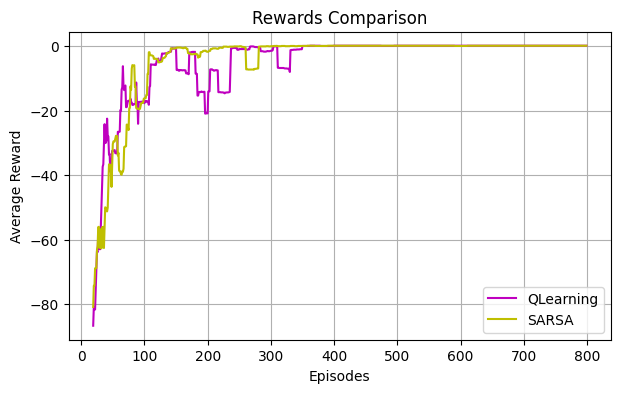
\includegraphics[width=0.4\textwidth]{rewards.png}}
\caption{Average rewards of Q-learning and SARSA}
\label{fig-reward}
\end{figure}

In Figure \ref{fig-reward}, the reward convergence of Q-Learning and SARSA follows a similar trend, with both algorithms experiencing rapid improvement in the early episodes. SARSA demonstrates a smoother learning curve, stabilizing slightly earlier than Q-Learning. In contrast, Q-Learning exhibits more fluctuations, indicating a greater degree of exploration. After approximately 300 episodes, both methods achieve near-optimal performance, with average rewards converging close to zero.

\begin{figure}[htbp]
\centerline{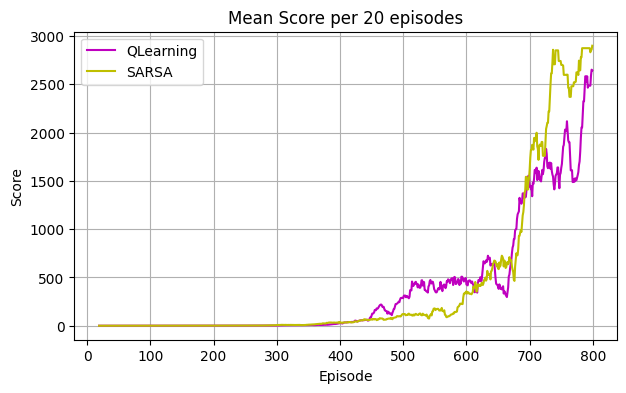
\includegraphics[width=0.4\textwidth]{scores.png}}
\caption{Mean score of Q-learning and SARSA}
\label{fig-score}
\end{figure}

Figure \ref{fig-score} illustrates the mean score progression of Q-Learning and SARSA over 800 episodes. Q-Learning learns faster in the mid-phase (400-600 episodes), while SARSA stabilizes more gradually. In the final phase (700+ episodes), SARSA surpasses Q-Learning, achieving higher peak scores with less fluctuation. Furthermore, Figure \ref{fig-gift} shows the gift collection efficiency of Q-Learning and SARSA over 800 episodes. SARSA learns to collect gifts earlier, but Q-learning catches up and achieves a similar capture rate (0.7 gifts per score) in later episodes. This indicates that SARSA learns to collect gifts earlier, but both can optimize the gift collection strategy in the long run.

\begin{figure}[htbp]
\centerline{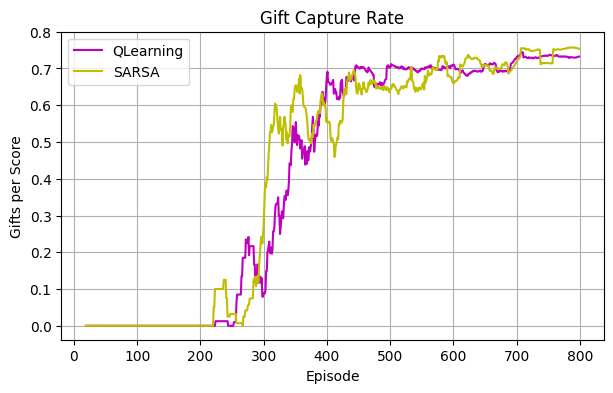
\includegraphics[width=0.4\textwidth]{gift_rate.png}}
\caption{Gift capture rate of Q-learning and SARSA}
\label{fig-gift}
\end{figure}



\section{Discussion and Conclusion}
\subsection{Discussion}
The results demonstrate that SARSA and Q-Learning exhibit distinct learning behaviors in training a Flappy Bird agent. SARSA shows more stable learning, achieving consistent rewards, higher peak scores, and earlier gift collection efficiency. In contrast, Q-learning learns faster initially but experiences greater fluctuations, reflecting its off-policy nature and tendency for broader exploration. Despite SARSA’s early advantage in gift collection, Q-learning eventually optimizes its strategy, leading to a similar gift capture rate. In long run, both algorithms converge towards effective policies.

\subsection{Limitations and Future Work}
While the results are promising, several limitations remain:
\begin{itemize}
    \item The discretization of continuous states might omit some dynamic details of the game.
    \item Further parameter tuning may improve performance.
    \item Future work could explore more complex reward structures and advanced state representation techniques, possibly incorporating deep learning methods.
\end{itemize}

\subsection{Conclusion}
The study compares Q-Learning and SARSA in training a Flappy Bird agent, highlighting their distinct learning behaviors. Besides, both algorithms demonstrate their effectiveness in this task given sufficient training conditions.

%\begin{thebibliography}{9}
%    \bibitem{sutton-barto}
%      Sutton, R. S. and Barto, A. G.,
%      \textit{Reinforcement Learning: An Introduction}.
%      MIT Press, 2018.
%    
%    \bibitem{mnih2015human}
%      Mnih, V., Kavukcuoglu, K., Silver, D., Rusu, A. A., et al.,
%      ``Human-level control through deep reinforcement learning,''
%      \textit{Nature}, 518(7540), 529--533, 2015.
%\end{thebibliography}

\end{document}
